% TU Delft Beamer template
% Author: Maarten Abbink
% Delft University of Technology
% March 2014
% Version 2.0
% Based on original version 1.0 of Carl Schneider
\documentclass{beamer}
\usepackage[english]{babel}
\usepackage{calc}
\usepackage[absolute,overlay]{textpos}
\usepackage{multicol}
\mode<presentation>{\usetheme{tud}}

\title[BEPStore]{BEPStore - Final Presentation}
%\subtitle
\institute[TU Delft]{Delft University of Technology}
\author{Bart Heemskerk, Wouter Kooyman van Guldener \& Steffan Sluis}
\date{\today}

% Insert frame before each subsection (requires 2 latex runs)
\AtBeginSection[] {\begin{frame}<beamer>\frametitle{\titleSubsec}
	    \begin{multicols}{2}
		\tableofcontents[currentsection,currentsubsection]  % Generation of the Table of Contents
		\end{multicols}
	\end{frame}
}
% Define the title of each inserted pre-subsection frame
\newcommand*\titleSubsec{Up next}
% Define the title of the "Authors" frame
\newcommand*\titleAuthors{About us}
% Define the title of the "Table of Contents" frame
\newcommand*\titleTOC{Outline}
% Define the title of the "End" frame
\newcommand*\titleEnd{Happy BEP'ing\!}

% define a symbol which can be removed if you don't need it
\newcommand{\field}[1]{\mathbb{#1}}
\newcommand{\Zset}{\field{Z}}

\begin{document}

{
% remove the next line if you don't want a background image
\usebackgroundtemplate{
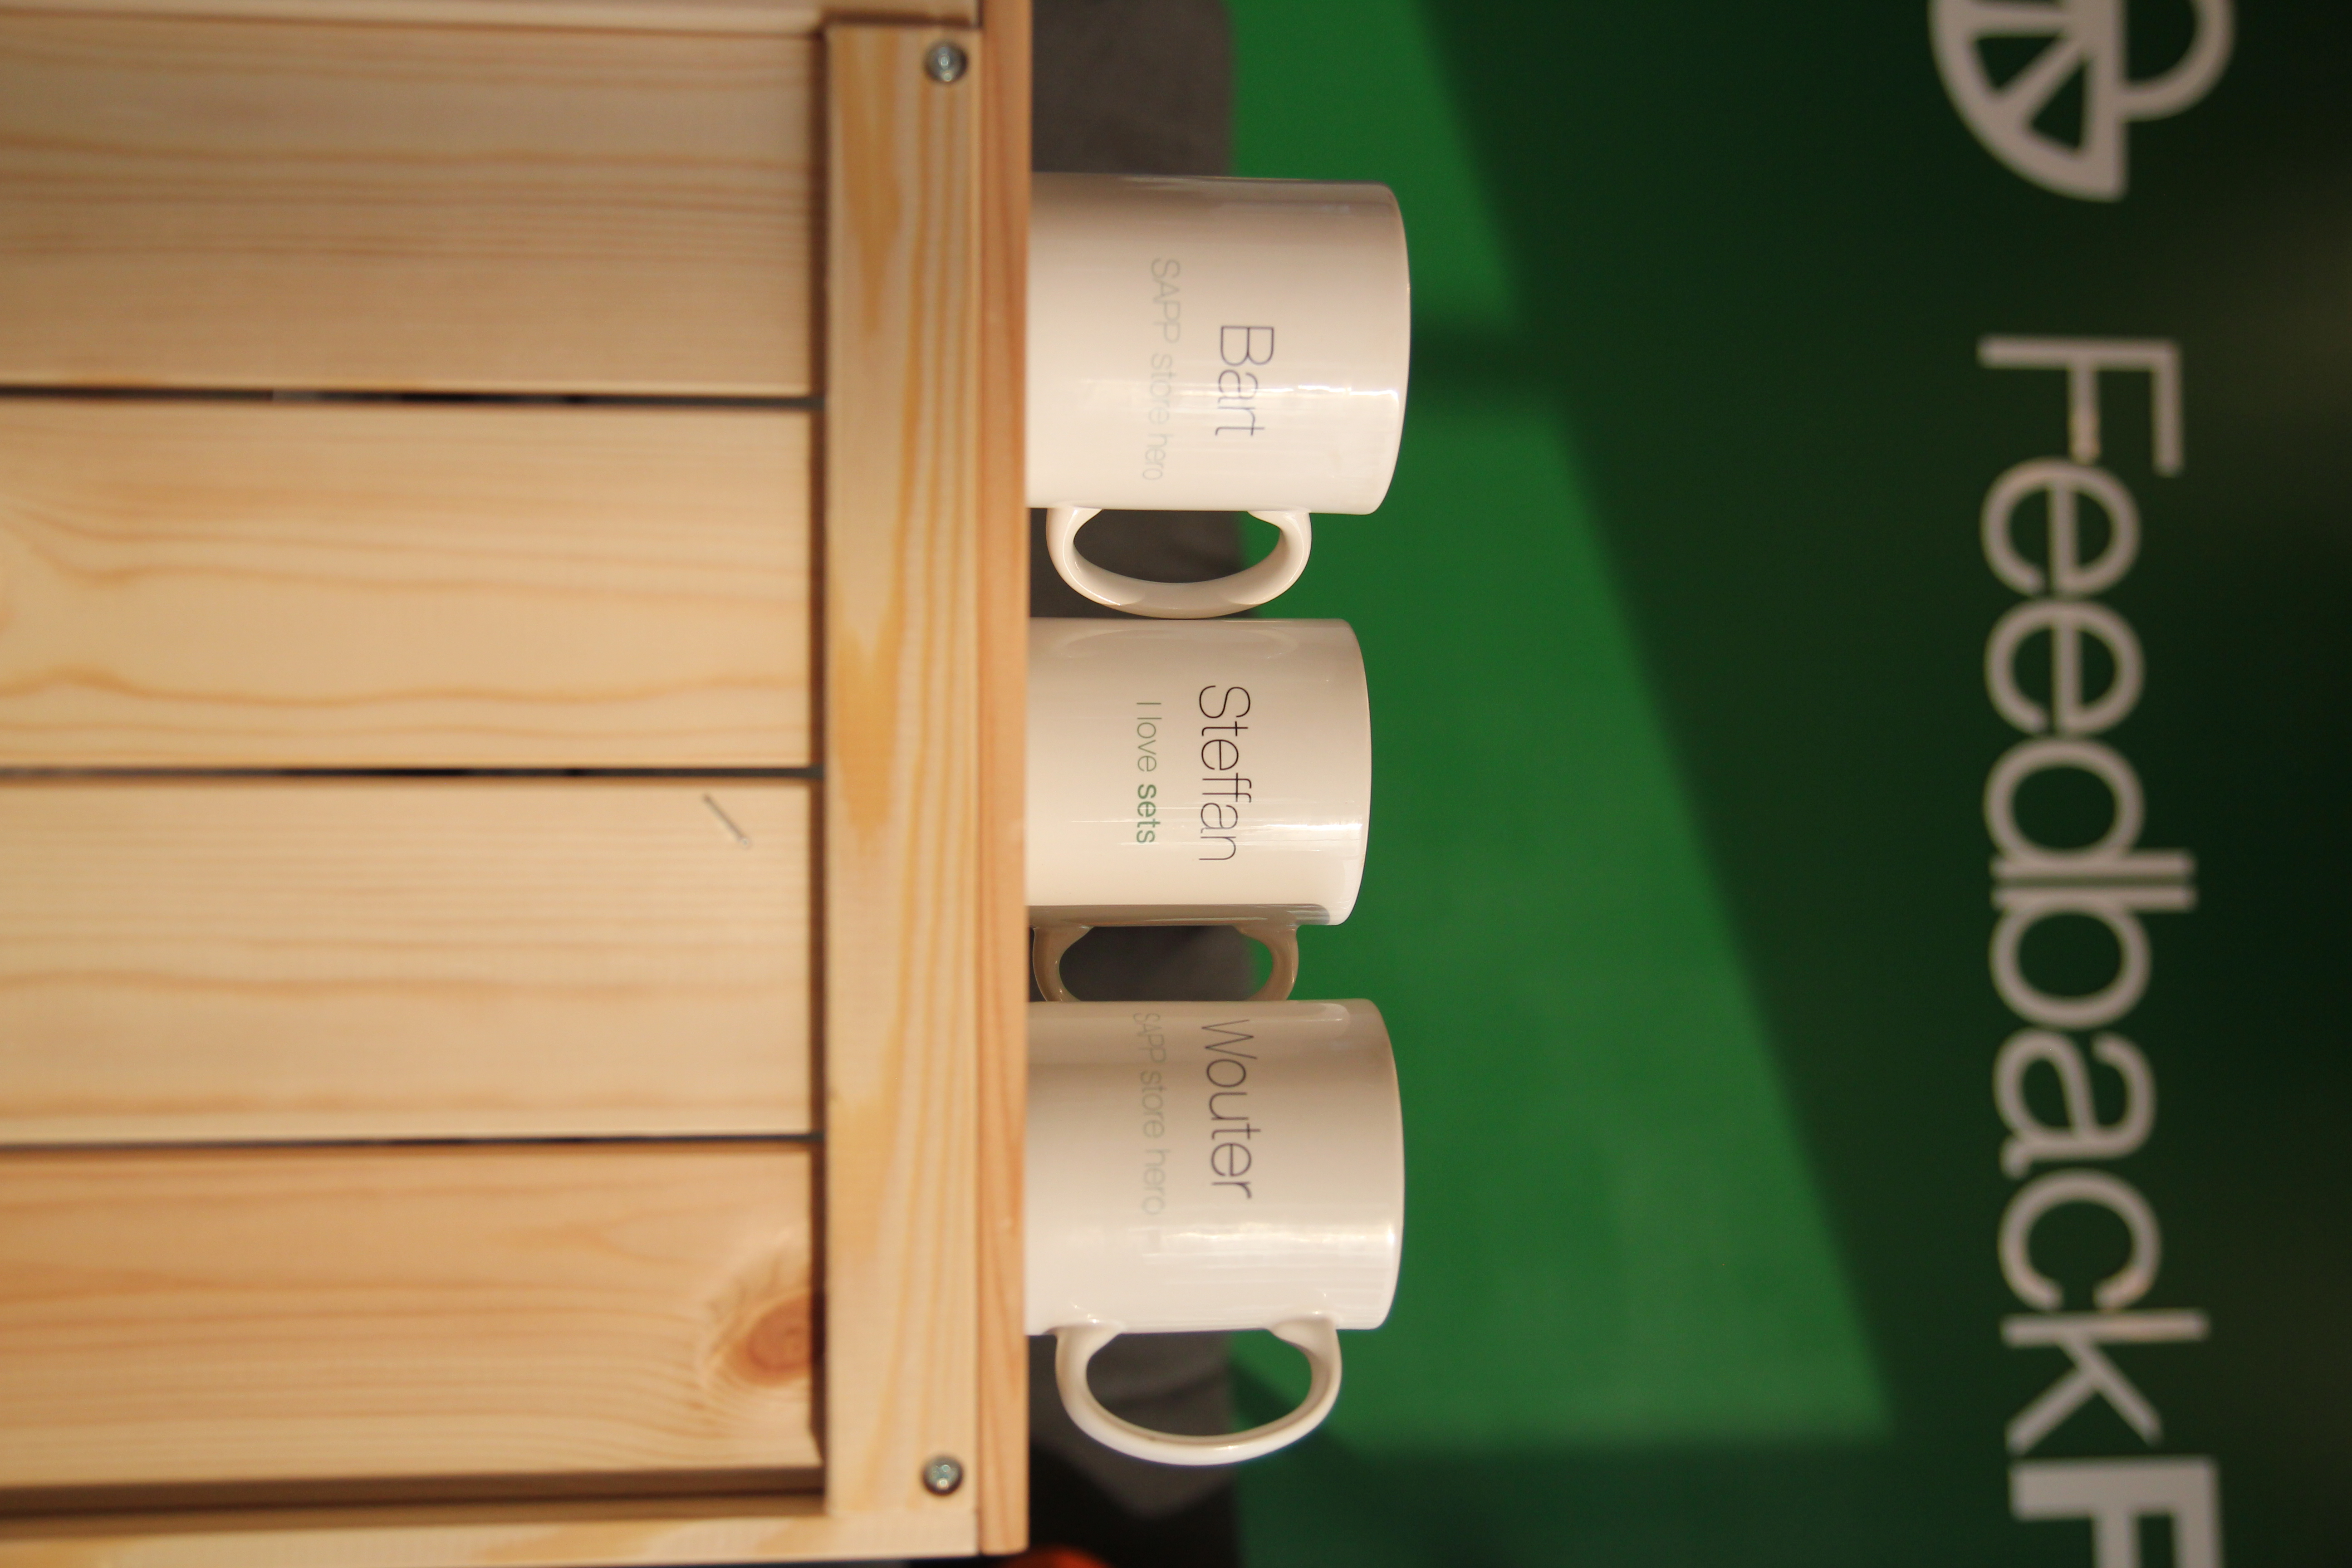
\includegraphics[height=\paperwidth,angle=90,keepaspectratio,trim=-0 0 7.5cm 0]{media/background}}%
\setbeamertemplate{footline}{\usebeamertemplate*{minimal footline}}
\frame{\titlepage}
}


{\setbeamertemplate{footline}{\usebeamertemplate*{minimal footline}}
\begin{frame}\frametitle{\titleAuthors}
    \begin{multicols}{3}
    % \includegraphics[width=1cm,keepaspectratio]{media/steffan}
    % Bart Heemskerk
    
    % \includegraphics[width=1cm,keepaspectratio]{media/steffan}
    % Wouter Kooyman van Guldener
    
    \centering{
    
        \begin{figure}[ht!]
            \includegraphics[width=2cm,keepaspectratio]{media/steffan}
            \label{fig:goal-design}
        \end{figure}
    
        Bart
    }
    
    \centering{
    
        \begin{figure}[ht!]
            \includegraphics[width=2cm,keepaspectratio]{media/wouter}
            \label{fig:goal-design}
        \end{figure}
    
        Wouter
    }
    
    \centering{
    
        \begin{figure}[ht!]
            \includegraphics[width=2cm,keepaspectratio]{media/steffan}
            \label{fig:goal-design}
        \end{figure}
    
        Steffan
    }
\end{multicols}

\vspace{2cm}

\centering{We have Twitter! @FBFBepstore}
\end{frame}
}


{\setbeamertemplate{footline}{\usebeamertemplate*{minimal footline}}
\begin{frame}\frametitle{\titleTOC}
    \begin{multicols}{2}
	    \tableofcontents
	\end{multicols}
\end{frame}
}

\section{Introduction}

\subsection{Client}

\begin{frame}\frametitle{Client}
    \begin{figure}[ht!]
        \centering
        \includegraphics[width=0.8\textwidth]{./media/feedbackfruits-logo}
        % \caption{The design for viewing a single goal}
        \label{fig:goal-design}
    \end{figure}
\end{frame}


% Small company, aimed at improving eduction by innovating software
\subsection{Subject \& motivation}
\begin{frame}\frametitle{Subject \& motivation}
    \begin{enumerate}
        \item User feedback
        \item Open-source developers
        \item Different toolsets
        \item Unification
    \end{enumerate}
\end{frame}
%1. Users have feedback but are mostly non-techinal,
%2. and developers lack domain knowledge.
% Open source is rising, knowledge gap between those two groups
%3. Users and developers use different toolsets.
%4. How to let these groups work together?

% Users of the clients platform are mostly non-technical people. The research report identifies GitHub as the most important tool for developers in the collaborative software development process. This tool focuses on developers and is not designed to be used by non-technical users. While the users would like to improve the clients platform, it appears to be difficult to translate their ideas to the developers because of a knowledge gap. The research conducted during this project shows that there are no existing implementations of a solution to this problem. The solution should bridge this gap in knowledge. Therefore, the contextual problem description can be defined as: ``How can the existing platform be extended in such a way that everyone in the FeedbackFruits community can contribute to the software development process?''

% 1. Technical knowledge is not always properly translated into function
% In addition to collecting feedback from their users, FeedbackFruits would like to boost community-engagement in improving education. It is the goal of the company to improve education for as many people as possible. The motivation behind stimulating community engagement is to create a community-driven ecosystem for innovation in education.
\subsection{Problem}

\begin{frame}\frametitle{Problem - Description}
    \begin{alertblock}{Problem}
		\centering{``How can the existing platform be extended in such a way that everyone in the FeedbackFruits community can contribute to the software development process?''}
	\end{alertblock}
	
\end{frame}

% The solution should bridge this gap in knowledge. Therefore, the contextual problem description can be defined as: “How can the existing platform be extended in such a way that everyone in the FeedbackFruits community can contribute to the software development process?”

\begin{frame}\frametitle{Problem - Analysis}
	\begin{enumerate}
        \item What can be learned from existing (non-software) communities?
        \item What current efforts exists to involve the community in the software development process?
        \item How are requirements established and used in software development?
        \item What limitations does the existing FeedbackFruits ecosystem impose on the software?
    \end{enumerate}
\end{frame}

% To anwser the four main research questions, the report will have four sections. The first research question zooms in on what can be learned from (non-software) communities. Before theories can be defined about what can be learned from all sorts of communities, a definition must be established of what a community is. Because communities exist in different sizes, with different structures and on different platforms, a few of these communities will be analysed in section 1.
% Some ways to involve the community in building software may be composed based on the previous section. However, this research will probably not be the only attempt to involve a software community in building software. The second research question is therefore focussed on existing platforms where software communities are involved in one way or another in the software development process. Section 2 will focus on the structure of the existing software communities. The techniques used by those communities and the way that the development process engages the community will also be examined.+

% Software development in its current form has some methodologies to establish requirements for a (big) software development project. The third research question will take a better look at the dynamics of requirements. These requirements are the basis of how the software will be built and are therefore an essential part of the software development process. In section 3, a few of the methods wich are used to establish requirements will be described. The dynamics of the requirements, like management and implementation, will also be given a closer look.
% The first three research question focus on determining the critical attributes of the problem in a general sense. However, because these attributes have to be applicable on the current FeedbackFruits-platform, that platform may pose some limitations. With research question four, the structure of the FeedbackFruits-platform will be examined, as well as the extensiblity of the platform. The result of this research question can be found in section 4.

% The most important aspects to this problem were identified in the research report as being: hype,requirements engineering, code and process updates (appendixD, chapter 5). Hype is necessary togain supporters that are willing to work on processing the feedback or feature requested by a user. Tobetter understand the how the feature should work, the feedback should be decomposed into smallchallenges via requirements engineering. These challenges should be converted to working code. Thecontributors should be informed of the current status of the feature through process updates. Thisprovides a feedback loop that ensures the challenges are tackled correctly.
\section{Research}

\subsection{Communities}
\begin{frame}\frametitle{Communities}
    \begin{enumerate}
        \item Goals
        \item Ideals
        \item Satisfaction
    \end{enumerate}
\end{frame}
\subsection{Software development}
\begin{frame}\frametitle{Software development}
    \begin{enumerate}
        \item Small core team
        \item Github or similar system
        \item Modular code
        \item Combined peer reviews and formal testing
        \item Stimulate intrinsic and extrinsic motivation
    \end{enumerate}
\end{frame}
\subsection{Requirements engineering}

\begin{frame}\frametitle{Requirements engineering}
    \begin{enumerate}
        \item Creating and managing requirements
        \item Decomposition into subproblems
        \item Iterative
    \end{enumerate}
\end{frame}
\subsection{FeedbackFruits ecosystem}
\begin{frame}\frametitle{FeedbackFruits ecosystem}
    \begin{enumerate}
        \item Architecture
        \item Software
        \item User experience
    \end{enumerate}
\end{frame}
\subsection{Conclusions}
\begin{frame}\frametitle{Conclusions}
    \begin{block}{Problem}
		\centering{``How can the existing platform be extended in such a way that everyone in the FeedbackFruits community can contribute to the software development process?''}
	\end{block}
	
	\begin{enumerate}
	    \item Time + knowledge = extensions
	    \item `With FeedbackFruits I would like to \ldots'
	    \item Goals, challenges and subchallenges
	    \item Supporters, hype and process updates
	    \item Tool integrations
	\end{enumerate}
\end{frame}

% The ideal platform should make it possible to convert resources in the form of time and knowledge into an extension to the current FeedbackFruits platform. The goal of this extension should be to fulfill a particular need. A goal can be identified as the answer to finishing the phrase: "With FeedbackFruits I would like to ..". Each goal can be divided in challenges, sub-goals that need to be met in order to meet the goal. If these challenges are to large to be solved by one or two supporters, then the challenges must be divided into sub-challenges in such a way that they can be solved by one or two pioneers. This implies that the whole project can be solved by lots of different people by tackling smaller problems at the same time.

% To attract these supporters it should be possible to hype a goal via, for example social media. To keep supporters in the loop it should also be possible to post process updates that get relayed to all supporters.

% The wheel should not be reinvented. Therefore integrations should be used wherever possible. Two examples:
% 1. GitHub: Used by many programmers.
% 2. Chat client. It is possible to make one ourselves, but is better to use an existing tool that people are already familiar with.
\section{Solution}

\subsection{Design}
\begin{frame}\frametitle{Design}
	\begin{enumerate}
	    \item Implements FeedbackFruits' architecture
	    \item Goal-centered
	    \item Engagement via social media
	    \item Integration with GitHub for developers
	    \item Realtime communication
	\end{enumerate}
	
% 	Plaatje Goals<-Supporters<-Social media <- GitHub
\end{frame}

\subsection{Challenges}
\begin{frame}\frametitle{Challenges}
	\begin{enumerate}
	    \item Planning
	    \item API standards
	    \item Shared codebase
	    \item Experimental web-technologies
	\end{enumerate}
	
% 	Plaatje Goals<-Supporters<-Social media <- GitHub
\end{frame}

% \subsection{Results}
% \begin{frame}\frametitle{Results}
% 	\begin{enumerate}
% 	    \item 
% 	\end{enumerate}
	
% % 	Plaatje Goals<-Supporters<-Social media <- GitHub
% \end{frame}

\subsection{Demo}
\begin{frame}\frametitle{Demo}
\begin{alertblock}{Demo}
		\centering{\Large{Demo}}
	\end{alertblock}
\end{frame}
\section{Conclusion}

\begin{frame}\frametitle{What was the problem again}
    \begin{alertblock}{Problem}
		\centering{``How can the existing platform be extended in such a way that everyone in the FeedbackFruits community can contribute to the software development process?''}
	\end{alertblock}
\end{frame}

\subsection{Accomplishments}
\begin{frame}\frametitle{Accomplishments}
    \begin{enumerate}
        \item Feedback solution
        \item Distributed problem solving
        \item Integration over reinvention
        \item Extensibility
    \end{enumerate}
\end{frame}
\subsection{Improvements}
\begin{frame}\frametitle{Improvements}
    \begin{enumerate}
        \item Planning
        \item More communication options
        \item Hype measurement
        \item Design contributions
        \item Contribution feedback
        \item Templates
    \end{enumerate}
\end{frame}
\subsection{Verification}

\begin{frame}\frametitle{Verification}
    \begin{figure}[ht!]
        \centering
        \includegraphics[width=0.8\textwidth]{./media/hackathon-graphic}
        \caption{by Clarus Commerce}
        \label{fig:goal-design}
    \end{figure}
\end{frame}

{\setbeamertemplate{footline}{\usebeamertemplate*{minimal footline}}
\begin{frame}\frametitle{\titleEnd}
    \subsection{Questions}

    \begin{figure}[ht!]
        \centering
        \includegraphics[width=0.6\textwidth]{./media/coffee_understands}
        \caption{by zazzle.nl}
        \label{fig:goal-design}
    \end{figure}

\end{frame}
}

% Include line below to see a sample
% \include{./sample}


\end{document}
